
The controller system’s architecture has been modelled such that the safety and liveness requirements are always met, by using the various sensors, actuators, and other components that are present in the system.

\section{Assumptions} 
The main assumptions about the system are as follows:
\begin{itemize}
    \item The robots perform the instructed actions without any error
    \item The lamp performs the projecting process without malfunctioning
    \item The other components may require the user to act upon them based on certain sensor data. To be precise,
    \begin{itemize}
        \item the airlock doors may not work
        \item the input stacks may become empty, and 
        \item the output stacks may become full
    \end{itemize}
\end{itemize}

However, to keep our model simple, we assume that the user intervenes where necessary and repairs the door(s), refills the input stack(s), and clears the output stack(s) as and when required. Thus, we have not included the user's actions in the model.

\section{System Architecture}
\begin{figure}[h]
\centering
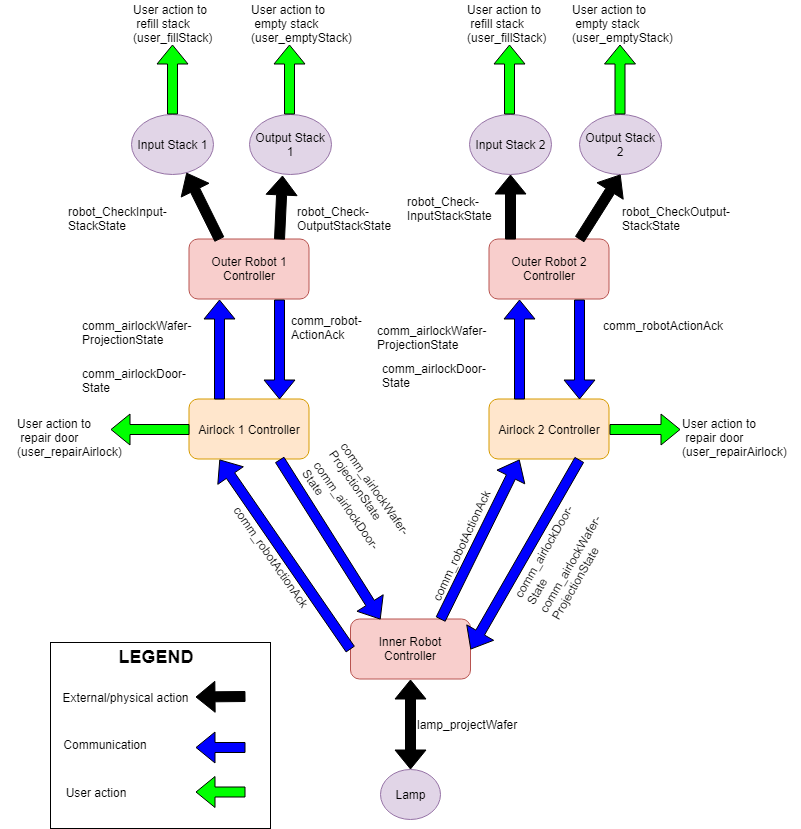
\includegraphics[width=150mm]{img/sv-project-arch.png}
\caption{System architecture diagram\label{fig:arch}}
\end{figure}

The architecture of the system is represented graphically using the Figure~{\ref{fig:arch}}. It consists of several controllers working in parallel to meet the requirements stated in chapter~{\ref{chap:reqs}}. The distribution of the above mentioned controllers is as follows:

\begin{itemize}
%    \item 2 input stack controllers
%    \item 2 output stack controllers
    \item 2 outer robot controllers
    \item 2 airlock controllers
    \item 1 inner robot controller
%    \item 1 lamp controller
\end{itemize}

For the most part, the system is expected to function without the need for any user input, but certain cases have been identified in which external "user interactions" are needed to meet the system’s liveness requirements. These are indicated by green arrows in the diagram (but as stated in the assumptions section, they are assumed to be performed immediately as needed).

All physical actions of the system are modelled as external interactions (as stated in the requirements chapter, chapter~{\ref{chap:reqs}). They are represented in the architecture diagram using black arrows.

There are various controllers for the components, and communication between the controllers is represented using blue arrows in the architecture diagram. These interactions take place between the controllers continuously and ensure that the system runs automatically. The controllers send the state of their associated components and poll for the states of other components as required, and make state transitions by performing the appropriate actions. The state transitions should not end up causing a deadlock within the overall system, at any cost.

There are some \textit{passive} components as well that are not controllers but are needed for the system's functioning - the stacks and the lamp. These are indicated in the architecture diagram too, since the controllers make use of them through external actions to signify relevant physical actions.

The system never reaches a state of “completion” since it is expected to run continuously till one of the conditions requiring an external \textit{user interaction} is met. Theoretically, if the user continually replenishes the input stack with new wafers and clears the output stack at the same rate, and if the airlock doors do not malfunction, the system can run for an indefinite period of time.
